%\title{18W MOSFET amplifier)
% Title: 18W MOSFET amplifier, with npn transistor.
% Author: Ramón Jaramillo.
% Source: http://www.circuitstoday.com/mosfet-amplifier-circuits
% Abstract:
% This example made use of circuitikz and siunits packages for drawing a 18W MOSFET  Amplifier for one-channel. It is mandatory than siunitx and related packages have been instaled, acording to your LaTeX distribution.
\documentclass[10pt,a4paper]{standalone}
\usepackage[utf8]{inputenc}
\usepackage{amsmath}
\usepackage{amsfonts}
\usepackage{amssymb}
\usepackage[,european]{circuitikz}
\usepackage{amsmath}
\begin{document}
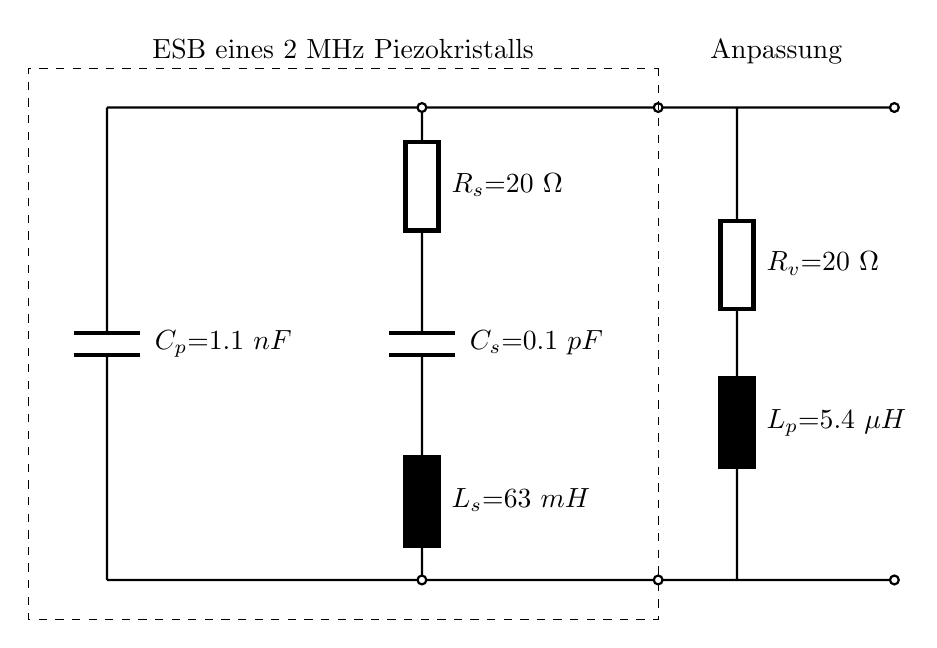
\begin{tikzpicture}[scale=2] 
\draw[color=black, thick]
	(0,0) 	to [C=\ $C_p{=}1.1\ nF$] (0,-1)
	(2,1) 	to [R=\ $R_s{=}20\ \Omega$] (2,0)
			to [C=\ $C_s{=}0.1\ pF$] (2,-1)
			to [L=\ $L_s{=}63\ mH$] (2,-2)

	(4,0.5)	to [R=\ $R_v{=}20\ \Omega$] (4,-0.5)
			to [L=\ $L_p{=}5.4\ \mu H$] (4,-1.5)

	(2,1)	to [short, o-o] (3.5,1)
	(0,1)	to [short, -] (2,1)
	(0,0)	to [short, -] (0,1)
	(0,-1)	to [short] (0,-2)
%	(-1,-2)	to [short, -] (0,-2)
	(0,-2)	to [short, -] (2,-2)
	(2,-2)to [short, o-o] (3.5,-2)
	
	(3.5,1)	to [short, -o] (5,1)
	(4,1)	to [short, -] (4,0.5)
			
	(3.5,-2)to [short, -o] (5,-2)
	(4,-2)	to [short, -] (4,-1.5)
	(1.5,1.5)  node[below] {ESB eines 2 MHz Piezokristalls}
	(4.25,1.5)  node[below] {Anpassung}
;
\draw[dashed]
   (3.5,1.25) 	-- (3.5,-2.25)
   			-- (-0.5,-2.25)
   			-- (-0.5,1.25)
   			-- (3.5,1.25)
;


%	(0,-0.5) node[transformer core] (T) {}
%	(T.A1) node[anchor=east] {$IN^+$}
%	(T.A2) node[anchor=east] {$IN^-$}
%	(T.B1) node[anchor=west] {B1}
%	(T.B2) node[anchor=west] {B2}
%	(T.base) node{K}
%	(0,-1) to [C=1<\farad>] (2,0)
	
%	(1.5,-0.25) to [sDo] (0.5,-0.25)
%				to [short, -o] (0.5,0){}
%				to [short] (0.5,0.25){}
%				to [sDo] (1.5,0.25)
%				to [short, -o] (1.5,0){}
%				to [short] (1.5,-0.25){}
%	(1.5,0)		to [short] (1.75,0){}
%	(1.75,0) 	to [short, o-o] (4.25,0)
%	(2,0) 	to [R=\ $R_i$] (2,-1)
%				to [short] (2,-2.1)
%	(2.75,0) 	to [C=\ $C_0$] (2.75,-1)
%				to [short] (2.75,-2.1)
%	(3.5,0) 	to [L=\ $L$] (3.5,-1)
%				to [C=\ $C$] (3.5,-2.1)
%	(1.75,-2.1)	to [short, o-o] (4.25,-2.1)
	% Output
%         (6,3) to [pC, l=$C_5$,-*](5,3)
%         (6,3) to [short,-o] (6,2){}
%         (6,0) to [short,-o] (6,1){} node[above=7mm]{\large{\textbf{SPEAKER}}}
 %        ;
%\draw[dashed]
  % (1.75,0.5) -- (1.75,-2.5)
   %(4.25,0.5) -- (4.25,-2.5)
%   ;
\end{tikzpicture}
\end{document}